\section{Sampling Theorem}

To obtain a discrete-time signal from a continuous-time signal, we need a \textbf{C/D converter}.
 \begin{figure}[H]\centering
 \includegraphics[width = 0.4\textwidth]{images/cdconverter}
 \caption{C/D converter} \end{figure}
 \ \\
The mathematical expression for a C/D converter is:
\[ x[n] = x_{c}(nT) \quad -\infty < n < +\infty \]
\ where $T$ is sampling period, $f_{s} = \frac{1}{T}$ is sampling frequency. 
\begin{itemize}
\item In general, the C/D transformation cannot be inverted.
\item Infinite continuous signals can reproduce a given sequence of samples,
\end{itemize}
An ideal C/D converter applies $T$ property, so that the sampling can be done without loosing information. 

%-------------------Sampling Process---------------------%
\subsection{Sampling Process}
Impulse train modulator $s(t)$ is: 
\[ s(t) = \sum_{-\infty}^{+\infty} \ \delta(t-nT) \]
The sampled signal $x_{s}(t)$ is obtained by multiplying the impulse train modulator by the continuous-time signal $x_{c}(t)$:
\begin{align*} 
\begin{split}
x_{s}(t) &= x_{c}(t) \ s(t)\\
&= \sum_{n=-\infty}^{+\infty} x_{c}(t) \delta(t-nT)\\
&= \sum_{n=-\infty}^{+\infty} x_{c}(nT) \delta(t-nT)
\end{split}
\end{align*}
Sampled signal, $x_{s}(t)$, is still defined in continuous-time, but it contains all information in the sampled discrete-time domain.\\\\

\begin{minipage}{\textwidth}
\begin{wrapfigure}{r}{0.5\textwidth}
\includegraphics[width = 0.5\textwidth]{images/sampling1}
\caption{(a)Original signal;(b) Sampled signal } \end{wrapfigure}
Apply the Fourier transform to  $x_{s}(t)$:
\begin{align*} \begin{split}
X_{s}(\omega) &= \mathcal{FT}\{x_{c}(t)\} \cdot \mathcal{FT}\{s(t)\}\\
&=\frac{1}{2\pi} X_{c}(\omega) * \mathcal{FT}\{s(t)\} \\
&=\frac{1}{T} X_{c}(\omega) * \sum_{n=-\infty}^{+\infty} \delta (\omega - k \omega_{s})\\
&=\boxed{\frac{1}{T} \sum_{n=-\infty}^{+\infty}  X_{c}(\omega - k \omega_{s})}
\end{split} \end{align*}
where sampling frequency $\omega_{s}=\omega_{0}=\frac{2\pi}{T}$.
\end{minipage}
\ \\\\\\
For sampled signals: $\omega_{N}$ is the signal bandwidth
\begin{itemize}
    \item if $\omega_{s} \geq 2\omega_{N}$, the replicas in the periodization do not overlap
    \item if $\omega_{s} < 2\omega_{N}$, the replicas overlap, also known as \textbf{aliasing}\footnote{``alias" is a Latin word, meaning ``otherwise", or ``elsewhere".}.
\end{itemize} 

\begin{figure}[H]\centering
\includegraphics[width = 0.6\textwidth]{images/sampling2}
\caption{(c) $\omega_{s} \geq 2\omega_{N}$; \ (d) aliasing: $\omega_{s} < 2\omega_{N}$} \end{figure}

%-------------------Reconstruction Process---------------------%
\subsection{Reconstruction Process}
Ideal low-pass filters can be used to reconstruct the signals.
\begin{figure}[H]\centering
\includegraphics[width = 0.5\textwidth]{images/lowpass}
\caption{Low-pass filter system} \end{figure}

\begin{figure}[H]
\begin{minipage}{0.6\textwidth}
1. Multiply the sampled signals by the function $H_{r}(\omega)$ \\
\[ X_{c}(\omega) = X_{s}(\omega) \cdot H_{r}(\omega) \]
\end{minipage} \hfill
\begin{minipage}{0.5\textwidth}
\includegraphics[width = \textwidth]{images/homega}
\caption{$H_{r}(\omega)$}
\end{minipage}\end{figure}

\begin{figure}[H]
\begin{minipage}{0.65\textwidth}
2. Due to the convolution property:
\[ X_{c}(\omega) = \mathcal{FT} \{  x_{s}(t) * h_{r}(t) \} \]
3. Apply inverse Fourier transform:
\begin{align*} \begin{split}
 x_{c}(t)&= x_{s}(t) * h_{r}(t) \\
 &=\sum_{n=-\infty}^{+\infty} x_{c}(nT) \delta(t-nT) * h_{r}(t)\\
 &=\boxed{\sum_{n=-\infty}^{+\infty} x_{c}(nT) h_{r}(t-nT)}\\\\
 &=\sum_{n=-\infty}^{+\infty} x_{c}(nT) \frac{\sin(\pi(t-nT) / T)}{\pi(t-nT) / T}
\end{split}\end{align*}
with \[ h_{r}(t)=\frac{\sin(\pi t/T)}{\pi t/T} \]
\end{minipage} \hfill
\begin{minipage}{0.35\textwidth}
\includegraphics[width = \textwidth]{images/reconstruction2}
\caption{Reconstruction}
\end{minipage}
\end{figure}

%-------------------Nyquist-Shannon Sampling Theorem---------------------%
\subsection{Nyquist-Shannon Sampling Theorem}
Nyquist-Shannon sampling theorem states that: \textbf{to retain the ability to reproduce (reconstruct) the original signal, the minimum sampling frequency during signal sampling must be at least twice its frequency.}\\

Mathematically, let $x_{c}(t)$ be a band-limited signal with $X_{c}(\omega)=0$, for $\lvert \omega \rvert \geq \omega_{N}$. Then $x_{c}(t)$ is uniquely determined by its samples $x[n] = x_{c}(nT)$, if 
\[ \omega_{s}=\frac{2\pi}{T} \geq 2\omega_{N} \]
where $2\omega_{N}$ is the minimal sampling rate and referred to as the \textbf{Nyquist rate}.\\

Nyquist-Shannon sampling theorem provides the condition under which the C/D transformation \textbf{can be inverted} without losing information, as shown in \autoref{fig:nyquist}.

\begin{figure}[H]
    \centering
    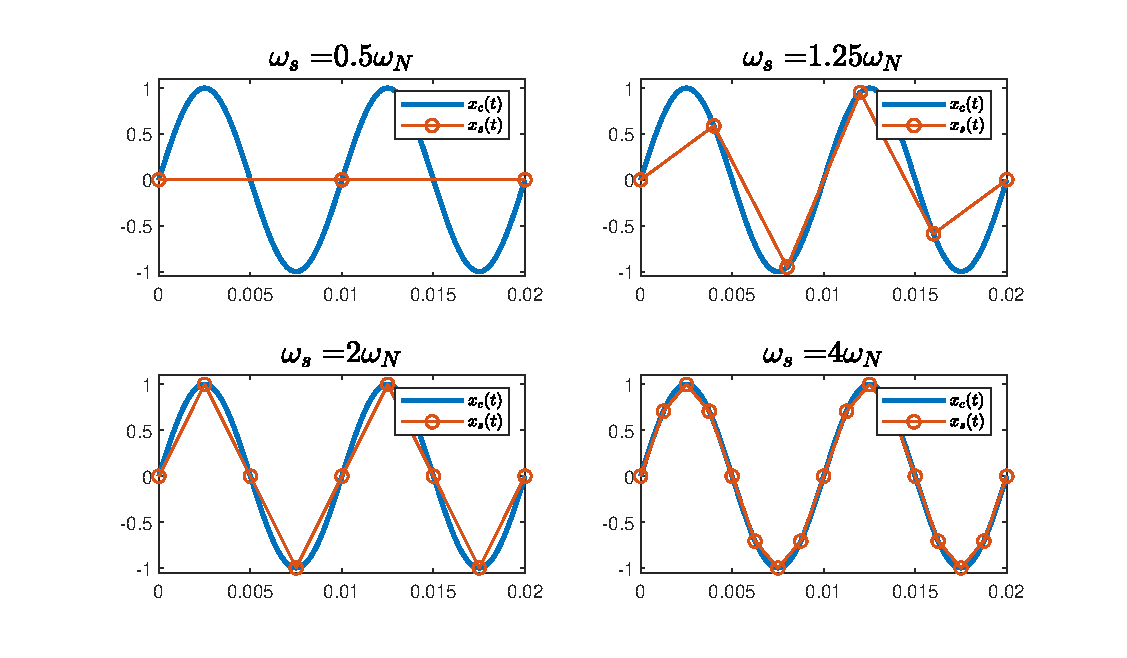
\includegraphics[width=\textwidth, center]{images/nyquist.eps}
    \caption{Sampling of a continuous signal $x_{c}(t)=\sin(200\pi t)$: (left to right, top to bottom) $\omega_{s}=0.5\omega_{N}$, $\omega_{s}=1.25\omega_{N}$, $\omega_{s}=2\omega_{N}$, $\omega_{s}=4\omega_{N}$. According to the Nyquist-Shannon sampling theorem, aliasing occurs when $\omega_{s} < 2\omega_{N}$}
    \label{fig:nyquist}
\end{figure}